\documentclass[12pt, twoside]{article}
\usepackage[letterpaper, margin=1in, headsep=0.5in]{geometry}
\usepackage[english]{babel}
\usepackage[utf8]{inputenc}
\usepackage{amsmath}
\usepackage{amsfonts}
\usepackage{amssymb}
\usepackage{tikz}
%\usetikzlibrary{quotes, angles}

\usepackage{graphicx}
\usepackage{enumitem}
\usepackage{multicol}

\usepackage{fancyhdr}
\pagestyle{fancy}
\fancyhf{}
\renewcommand{\headrulewidth}{0pt} % disable the underline of the header

\fancyhead[RE]{\thepage}
\fancyhead[RO]{\thepage \\ Name: \hspace{3cm}}
\fancyhead[L]{BECA / Dr. Huson / 10th Grade Geometry\\* Unit 7: Analytic Geometry Review\\11 February 2019}

\begin{document}
\subsubsection*{Do Now: Distance on the coordinate plane}
  \begin{enumerate}
    \item Given right $\triangle JKL$ with $\overline{JK} \perp \overline{KL}$, $JL=13$, and $JK=12$.
    \begin{enumerate}

      \item Find the length $KL$. \vspace{1cm}

        \begin{center}
          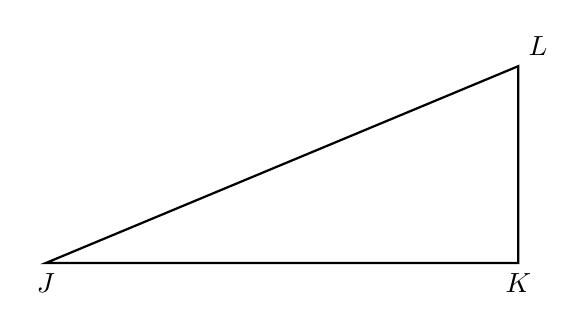
\begin{tikzpicture}[scale=0.5]
            \draw [thick]
            (0,0) node[below]{$J$}--
            (12,0)  node[below]{$K$}--
            (12,5) node[above right]{$L$}--cycle;
          \end{tikzpicture}
        \end{center}
        \vspace{1cm}
    Based on the triangle above, express each trigonometric value as a fraction.\\
    \item $\sin J=$ \vspace{0.5cm}
    \item $\cos J=$ \vspace{0.5cm}
    \item $\tan J=$  \vspace{1.5cm}
  \end{enumerate}

    \item Convert this quadratic function from vertex form to standard form ($f(x)=x^2+bx+c$) by expanding the squared term and simplifying.

        \[f(x) = (x-5)^2-1\]
\newpage

\item Regent problem: Line segment $A'B'$, whose endpoints are $(4,-2)$ and $(16,14)$, is the image of $\overline{AB}$ after a dilation of $\frac{1}{2}$ centered at the origin. What is the length of $\overline{AB}$? \vspace{5cm}

\item Regent problem: \\
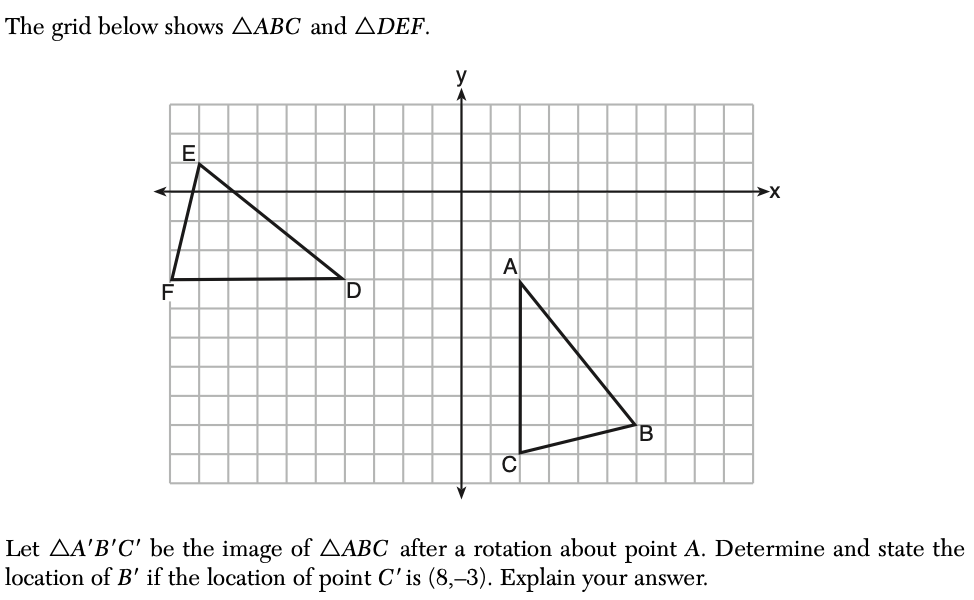
\includegraphics[width=15cm]{7-9rotation.png}


\end{enumerate}

\newpage

\subsubsection*{Classwork: Algebra efficient solutions}
\begin{enumerate}
  \item Solve each problem two ways: as a first step distribute, and as a first step multiply each side of the equation by the fraction's denominator. \vspace{0.5cm}
  \begin{multicols}{2}
    \raggedcolumns
    \begin{enumerate}
  \item   $\frac{1}{2}(4x-6)=3$ \vspace{2.5cm}
  \item   $\frac{1}{3}(5x-4)=2$ \vspace{2.5cm}
  \end{enumerate}

  \end{multicols}
  \vspace{13cm}
Which way is better? Explain
\newpage

\item To solve for $x$, what would be the best first step? \\[0.5cm]
Write down one of the following: distribute, multiply (both sides) by 5, multiply by $x$, multiply by 3, multiply by $\frac{3}{2}$, factor, substitute for $x$, collect like terms. \vspace{0.5cm}
\begin{multicols}{2}
  \raggedcolumns
  \begin{enumerate}
\item   $\frac{1}{5}(10x+5)=3$ \vspace{0.5cm}
\item   $\frac{2}{3}(5-x)=-4$ \vspace{0.5cm}
\item $x^2-4x+5x+4x^2-7=15$ \vspace{0.5cm}
\item $\frac{1}{3}(9x+3)=17$ \vspace{0.5cm}
\item $g(x)=x^2-5x+3$. Find $g(1)$. \vspace{0.5cm}
\item $x^2-4x-5=0$. \vspace{0.5cm}
\item $\displaystyle \sin 31^\circ = \frac{5}{x}$. \vspace{0.5cm}
\item $\displaystyle \cos 29^\circ = \frac{x}{5}$. \vspace{0.5cm}


\end{enumerate}
  \rule{6cm}{0.15mm} \\[0.75cm]
  \rule{6cm}{0.15mm} \\[0.75cm]
  \rule{6cm}{0.15mm} \\[0.75cm]
  \rule{6cm}{0.15mm} \\[0.75cm]
  \rule{6cm}{0.15mm} \\[0.75cm]
  \rule{6cm}{0.15mm} \\[0.75cm]
  \rule{6cm}{0.15mm} \\[0.75cm]
  \rule{6cm}{0.15mm}

\end{multicols}
\vspace{1.5cm}

  \item Write down the center and radius of each circle.
    \begin{enumerate}
      \begin{multicols}{2}
      \item   $(x-3)^2+(y-1)^2=16$ \vspace{2cm}
      \item   $(x+2)^2+(y-7)^2=3^2$
      \item   $(x-5)^2+y^2=121$ \vspace{2cm}
      \item   $(x+2)^2+(y-3)^2=9^2$
      \end{multicols}
    \end{enumerate}
    \vspace{0.5cm}

  \end{enumerate}

\newpage

\subsubsection*{Classwork: Distance on the coordinate plane}
  \begin{enumerate}

    \item Complete the t-chart for $x=-5,-4,-3,0,3,4,5$, then graph points on the grid below. Use pencil for graphs.

        \[y = \sqrt{25-x^2}\]

        What is the shape of a smooth curve through the points?
      \begin{center} %4 quadrant regents grid w T-Chart
      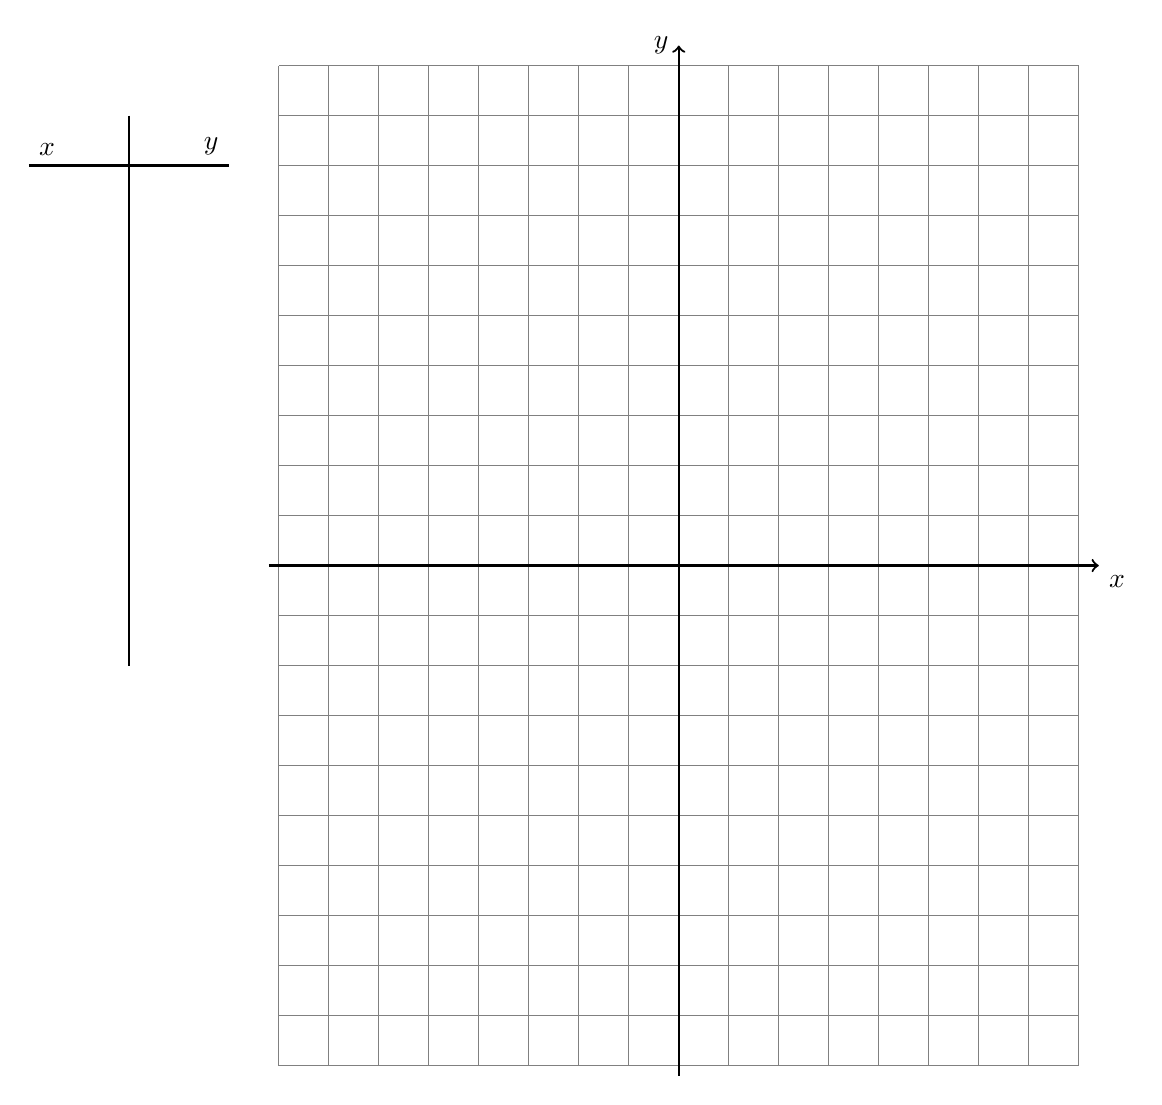
\begin{tikzpicture}[scale=.635]
        \draw [help lines] (-6,-10) grid (10,10);
        \draw [thick, ->] (-6.2,0) -- (10.4,0) node [below right] {$x$};
        \draw [thick, ->] (2,-10.2)--(2,10.4) node [left] {$y$};
        \draw [thick] (-11,8) node[above right]{$x$} --(-7,8) node [above left]{$y$};
        \draw [thick] (-9,9)--(-9,-2);
      \end{tikzpicture}
      \end{center}

    \begin{enumerate}
      \item Draw $\overline{OA}$ with $O(0,0)$ and $A(-3,4)$
      \item What is the length of $\overline{OA}$? \vspace{1.5cm}
    \end{enumerate}



\newpage

  \item On the set of axes below, graph the quadrilateral $ABCD$ having coordinates $A(-3,-3)$, $B(5,1)$, $C(6,8)$, and $D(-2,4)$.
    \begin{center} %4 quadrant regents grid
    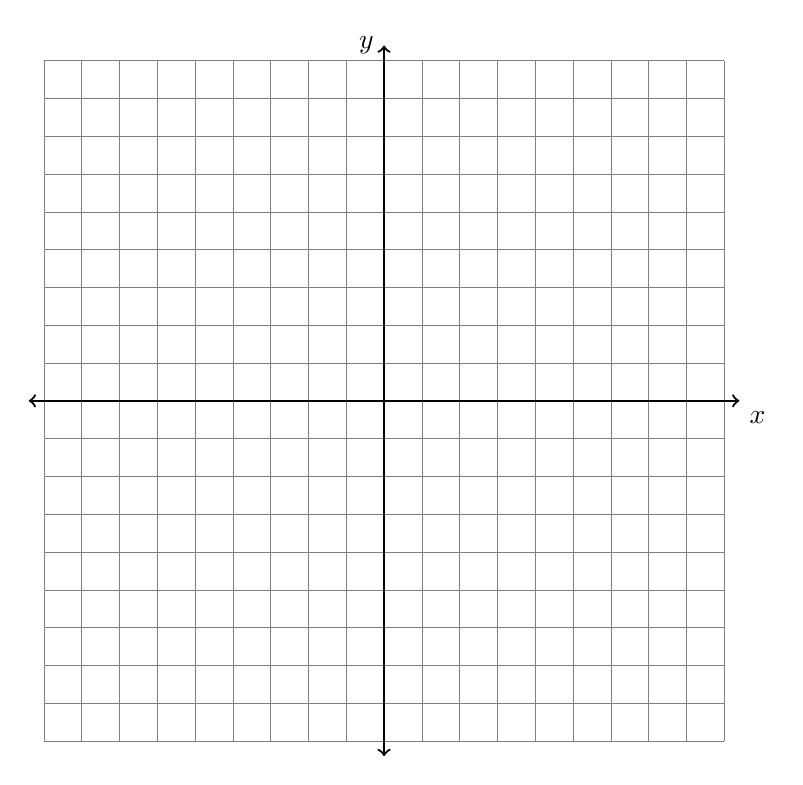
\begin{tikzpicture}[scale=.48]
      \draw [help lines] (-9,-9) grid (9,9);
      \draw [thick, <->] (-9.4,0) -- (9.4,0) node [below right] {$x$};
      \draw [thick, <->] (0,-9.4)--(0,9.4) node [left] {$y$};
      %\draw [thick] (-3,-3) node[below] {$A$}--
      %(5,1) node[right] {$B$}--
      %(6,8) node[left] {$C$}--
      %(-2,4) node[left] {$D$}--cycle;
      %\draw [fill] (5,0) circle [radius=0.1] node[above left] {$P$};
    \end{tikzpicture}
    \end{center}
    Find the length of each side of the quadrilateral.



  \end{enumerate}

  \end{document}
